\section{Testen}\label{sec: testen}

\subsection{Testroutine}\label{sec_routine}
\subsubsection{Rotationstest}
Der CubeSat, ein kleiner würfelförmiger Satellit, kann in einem Gyroskop befestigt werden, um die Stabilität und die Reaktionsfähigkeit des Satelliten auf Rotationsbewegungen in X-, Y-, und Z-Richtung zu testen. \\
\vspace{2mm}
Diese Rotationstests sind von wesentlicher Bedeutung, da sie es ermöglichen zu überprüfen, inwiefern der Satellit fähig ist, den komplexen Belastungen durch Rotation sowie anderen Bewegungen, denen er im Weltraum ausgesetzt ist, standzuhalten. Der Weltraum stellt eine äußerst anspruchsvolle Umgebung dar, in der Satelliten dynamischen Bewegungen, die insbesondere während des Manövrierens oder der Ausrichtung des Satelliten auftreten. Ein Schaden durch unkontrollierte oder nicht korrekt abgefangene Rotationsbewegungen könnte die Funktionstüchtigkeit des Satelliten erheblich beeinträchtigen und somit seine Mission gefährden. Durch die sorgfältige Durchführung dieser Tests vor dem Einsatz des Satelliten im Orbit lässt sich sicherstellen, dass dieser während seiner gesamten Einsatzzeit zuverlässig funktioniert und seine vorgesehenen Aufgaben erfüllen kann.


\subsubsection{Vibrationstest}
Der Vibrationstest ein unverzichtbarer Schritt, der dazu dient, die Widerstandsfähigkeit und Robustheit des Satelliten gegenüber den extremen Bedingungen während des Raketenstarts zu bewerten. Für diesen Test wird der CubeSat auf einer speziell konstruierten Rüttelplatte befestigt, die in der Lage ist, die intensiven Vibrationen zu simulieren, denen der Satellit beim Start ausgesetzt ist.\\
\vspace{2mm}
Diese Tests sind kritisch, da sie dazu beitragen, eventuelle Schwachstellen in der Struktur des CubeSats oder in seinen einzelnen Komponenten zu identifizieren, bevor er seine Mission im Weltraum antritt. Während des Vibrationstests werden nicht nur die strukturelle Integrität und die mechanische Belastbarkeit des CubeSats auf die Probe gestellt, sondern auch die Zuverlässigkeit der Sensoren auf dem CubeSat und anderer kritischer Systeme. \\
\vspace{2mm}
Die Erkenntnisse aus diesen Tests sind entscheidend, um festzustellen, wie gut der Satellit und seine Sensoren in der Lage sind, den Startbedingungen standzuhalten, ohne ihre Funktionsfähigkeit zu verlieren. Sollten die Tests Schwachstellen aufdecken, müssen notwendige Anpassungen vorgenommen werden. Diese können von der Verstärkung struktureller Komponenten bis hin zur Überarbeitung der Montage oder des Designs der Sensoren reichen, um die Missionstauglichkeit des CubeSats sicherzustellen. Letztendlich zielen Vibrationstests darauf ab, das Risiko eines Ausfalls während des kritischen Startvorgangs zu minimieren und die Erfolgschancen der Mission zu maximieren.


\subsubsection{Test im Vakuum}
Ein weiterer Test umfasst die Kombination von Vibrationstests mit der Simulation des Vakuums des Weltraums. Dies wird erreicht, indem der CubeSat auf einer Rüttelplatte platziert und zusätzlich eine Vakuumglocke verwendet wird. Diese Konfiguration ermöglicht es, gleichzeitig die mechanischen Belastungen des Starts und die Bedingungen des Weltraumvakuums zu simulieren.\\
\vspace{2mm}
Die Simulation des Weltraumvakuums ist kritisch, da sie Aufschluss darüber gibt, wie der Satellit und seine integrierten Systeme unter dem Einfluss eines nahezu vollständigen Vakuums operieren. Im Weltraum herrscht ein Druckniveau, das nahezu bei null liegt, was bedeutet, dass alle Materialien und Komponenten, die in der irdischen Atmosphäre entwickelt und getestet wurden, sich dort anders verhalten können. Insbesondere wird untersucht, wie gut die Materialien und elektronischen Komponenten des Satelliten diese Bedingungen tolerieren, ohne ihre Integrität oder Funktionalität zu verlieren.\\
\vspace{2mm}
Ein zentrales Anliegen dieser Tests ist die Überprüfung auf mögliche Lecks, die im Vakuum schneller auftreten können als unter irdischen Bedingungen.


\subsubsection{Einsatz von Sensoren}
Die Durchführung von Tests unter Einsatz von Sensoren, sowohl auf dem CubeSat selbst als auch in der Testumgebung, spielt eine entscheidende Rolle bei der Vorbereitung des Satelliten auf seinen Einsatz im Weltraum. Diese ermöglichen es, eine Vielzahl von Daten zu erfassen, die für die Bewertung der Leistungsfähigkeit und Zuverlässigkeit des CubeSats unter verschiedenen Simulationen bzw. Tests unerlässlich sind.

\subsubsection{UV-Lampe}
Um die anspruchsvollen und vielfältigen Bedingungen des Weltraums möglichst realitätsnah zu simulieren, ist es unerlässlich, neben Vakuum und Vibration auch die Auswirkungen der Sonnenstrahlung sowie die extremen Temperaturschwankungen, denen ein Satellit im Orbit ausgesetzt sein wird, zu testen. Die Verwendung einer UV-Lampe ermöglicht es, die intensive ultraviolette Strahlung der Sonne nachzubilden, der der CubeSat im Weltraum kontinuierlich ausgesetzt sein wird. Diese Simulation ist von entscheidender Bedeutung, da UV-Strahlung das Potenzial hat, elektronische Systeme zu beeinträchtigen und somit die Leistung und Lebensdauer des Satelliten signifikant zu reduzieren.\\
\vspace{2mm}
Zur Simulation der extremen Temperaturbedingungen, die im Weltraum herrschen, kommt ein Kühlgerät zum Einsatz. Im Weltraum durchläuft ein Satellit drastische Temperaturschwankungen. \\
\vspace{2mm}
Er ist hohen Temperaturen ausgesetzt, wenn er direkt der Sonne zugewandt ist, und erlebt gleichzeitig niedrige Temperaturen, wenn er sich im Schatten befindet. Diese Temperaturschwankungen können eine signifikante Belastung für die Struktur des Satelliten, seine Systeme und die an Bord befindlichen Instrumente darstellen. Materialien können sich ausdehnen oder zusammenziehen, was die strukturelle Integrität beeinträchtigen und zu Funktionsstörungen führen kann. Elektronische Komponenten sind besonders anfällig für Temperaturänderungen, die ihre Leistung beeinträchtigen oder sogar zum vollständigen Ausfall führen können.\\
\vspace{2mm}
Die Durchführung dieser Tests unter kontrollierten Bedingungen auf der Erde ist entscheidend, um sicherzustellen, dass der CubeSat und seine Systeme den extremen Bedingungen im Weltraum standhalten können.


\subsubsection{Fazit der Tests}
Die sorgfältige Durchführung dieser vielfältigen Tests ist von fundamentaler Bedeutung für die Vorbereitung des CubeSats auf seine Mission im Weltraum. Indem sie eine breite Palette an Umweltbedingungen simulieren, die im Weltraum vorherrschen, tragen diese Tests entscheidend dazu bei, die Zuverlässigkeit, Leistungsfähigkeit und Missionstauglichkeit des CubeSats zu gewährleisten.

\newpage

\SecAuth{\nameCZ}

\subsection{Messungen}\label{Messungen}
\subsubsection{Erklärung der Daten}
Um die Daten darzustellen und gegebenenfalls zu analysieren, müssen alle Daten zuerst fest definiert werden. Dazu sollte der Nutzen der Daten erklärt und alle Einheiten klargemacht werden. 

\subsubsection{Temperatur }
Auf dem EDU-Hat gibt es zwei Sensoren, welche akkurat die Temperatur des Raumes messen können. Der erste Sensor (TMP112) ist ein reiner Temperaturmesser, welcher die Temperatur in Grad Celsius zurückgibt. Auch der Gassensor (BME688) gibt die Temperatur akkurat in Grad Celsius an. \\
\vspace{3mm}
Das Messen der Temperatur ist für mögliche Experimente im All sehr wichtig. Eine Messung der Temperaturveränderung des CubeSats, um die Auswirkungen der Sonneneinstrahlung zu studieren, wäre hier ein gutes Experiment.\\
\vspace{3mm}
Weitere Informationen über die Sensoren können in Kapitel \ref{temperatur} gefunden werden.

\subsubsection{Messung des Magnetfeldes}
Der Magnetfeldsensor (BMM150 siehe Kap.: \ref{magentsen}) gibt seine Werte in einem kartesischen Koordinatensystem aus. Alle X, Y und Z Werte werden als µT (Micro-Teslas) zurückgegeben. Tesla ist die standardisierte Einheit für die magnetische Flussdichte. Das Magnetfeld der Erde besitzt am Äquator etwa 30 µT\autocite{Erdmagnetfeld}, während ein durchschnittlicher Magnet etwa 1T-1,5T besitzt.\\
\vspace{3mm}
Der Magnetfeldsensor dient zur Messung der Rotation des Satellites. Auch können mögliche magnetische Störungen vom Sensor, wie zum Beispiel magnetische Stürme oder das Magnetfeld der Erde, aufgenommen werden.\\
\vspace{3mm}
Signifikante Messergebnisse können möglicherweise durch den Einfluss eines externen Magneten in der Teststation gemessen werden.
\newpage
\subsubsection{Messung von Beschleunigung}
Wie in Kapitel \ref{beschleuni} schon erwähnt, werden die Werte des Beschleunigungssensors (ADXL345) in G-Kräften angegeben. Ein G entspricht der Erdanziehungskraft, während zum Beispiel 6G der sechsfachen Erdanziehungskraft entsprechen. \\
\vspace{3mm}
G-Kräfte können sich jedoch nicht nur auf die Gravitationskraft der Erde beziehen. Die Größe kann auch für die Beschleunigung eines Objekts verwendet werden. \\
\vspace{3mm}
Obwohl in der Teststation nur gyroskopische Effekte auf den Satelliten wirken, können eventuell mögliche Erschütterungen durch eine eingebaute Rüttelplatte gemessen werden. Sonstige Bewegungen müssen außerhalb der Teststation simuliert werden.

\subsubsection{Messung der UV-Strahlung}\label{messuv}
Der UV-Sensor (GUVA\_C32) welcher für die Messung einkommender UV-Strahlung verwendet wird, gibt bei der Auslesung zwei wichtige Werte zurück.\\
\vspace{3mm}
Der Wert UVA steht für Ultraviolettstrahlung vom Typ A. UVA-Strahlen haben eine Wellenlänge von 320-400 Nanometer.\\
\vspace{3mm}
Der UV-Index ist ein internationaler Index für die Messung der Stärke von UV-Strahlen. Der UV-Index berücksichtigt sowohl UVA-, als auch UVB-Strahlen und wird in einem Index von 0 bis 11+ skaliert, wobei 0 die niedrigste Stärke darstellt.\\
\vspace{3mm}
UVB-Strahlen stehen für Ultraviolettstrahlung vom Typ B. Diese Strahlen haben eine Wellenlänge von 280-320 Nanometer und sind hauptverantwortlich bei der Entstehung von Sonnenbrand und Hautkrebs.\\
\vspace{3mm}
Der Sensor ist besonders wichtig, um die Sonneneinstrahlung im Weltraum, wo die Strahlungsintensität um einiges höher ist als auf der Erdoberfläche, zu messen. 

\subsubsection{Messung der Luftfeuchtigkeit}
Für die Messung der Luftfeuchtigkeit ist der Gassensor (BME688) zuständig. Die Luftfeuchtigkeit ist der Anteil des gasförmigen Wassers, welcher sich in einem Raum, bzw. in der Atomsphäre, befindet. Dieser Anteil wird in Prozent angegeben und korreliert mit der Temperatur.\\
\vspace{3mm}
Der Feuchtigkeitssensor kann verwendet werden, um die Menge des Wasserdampfes in der oberen Atmosphäre zu messen. Somit kann der Sensor für verschiedene meteorologische Versuche verwendet werden. 

\newpage
\subsubsection{Messung des Luftdrucks}
Der Luftdruck wird ebenfalls über den BME688 gemessen. Der Luftdruck ist definiert als das Gewicht der Luft in der Erdatmosphäre. Je nach Höhe des Messvorgangs kann sich dieser Wert verändern. Der Luftdruck nimmt mit zunehmender Höhe des Satelliten ab. Der Luftdruck wird in der Einheit des Drucks (Pa - Pascal) angegeben. Bei der Testung des Systems sollte der Luftdruck bei einer Höhe von 461m (Höhe Rankweil) und bei einer Raumtemperatur von 25°C etwa 96080Pa sein.\\
\vspace{3mm}
Solch ein Sensor kann im Sensor verwendet werden, um Höheninformationen zu ermitteln. Auch können Änderungen des Luftdrucks wichtig für die Vorhersage von anstehenden Wetterveränderungen sein. 

\subsubsection{Messung der Luftqualität }
Der Gassensor (BME688) kann auch die Luftqualität in einem bestimmten Raum, bzw. Gebiet messen. Dazu wird der Wert der Gasbeständigkeit genutzt und in Ohm angegeben. Je höher die Gasbeständigkeit in einem Raum ist, desto besser ist die allgemeine Luftqualität.\\
\vspace{3mm}
Somit kann der Sensor auch für die Überprüfung der Carbon Emissionen von bestimmten Gebieten genutzt werden. 

\subsubsection{Messergebnisse der Sensoren}
Nachdem die Sensordaten erfolgreich über die Webanwendung (siehe Kapitel: \ref{Web}) ausgegeben und in einer visuell ansprechenden Weise dargestellt wurden, besteht die Möglichkeit, die Sensorik des EDUs eingehend zu prüfen. Diese Prüfung zielt darauf ab, die Funktionalität der Sensorik unter variierenden Umweltbedingungen zu testen. 

\subsubsection {Messergebnis Temperatur}
Beide Temperatursensoren messen die Temperatur bei einer Raumtemperatur von 28°C. Nach der Belüftung des Raumes, in dem sich der EDU befindet, wird erwartet, dass die von den beiden Temperatursensoren erfasste Temperatur sinkt. Dies ist eine direkte Folge der Abkühlung, die durch den Luftaustausch während des Lüftens verursacht wird.\\
\vspace{3mm}
\begin{figure}[H]
	\centering
	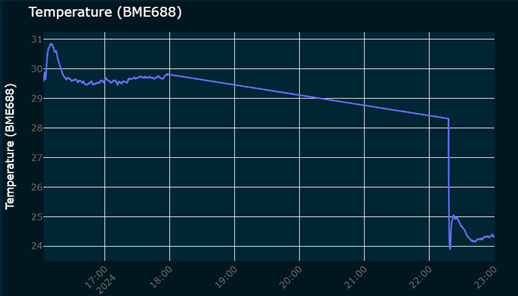
\includegraphics[scale = 1]{image/tempmess1.png}
	\caption{Messung Temperatur}
	\label{fig:enter-label}
\end{figure}
\vspace{3mm}
Zu sehen ist der Temperaturunterschied des Sensors BME688 (Kap.:\ref{temperatur}). Links im Diagramm ist die Raumtemperatur zu sehen. Anschließend wird das Fenster des Raumes geöffnet und die Temperatur sinkt. Die linear verlaufende Linie, die zwischen den zwei Temperaturunterschieden zu sehen ist, kennzeichnet, dass in diesem Zeitraum keine Datenaufnahme stattgefunden hat.
\vspace{3mm}
\begin{figure}[H]
	\centering
	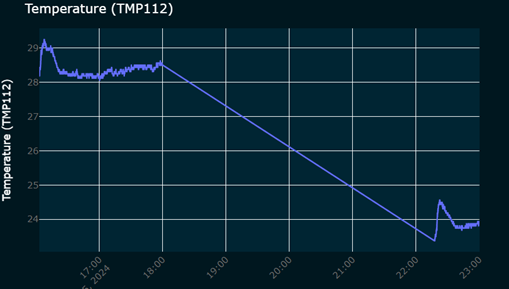
\includegraphics[scale=1]{image/temp2mess.png}
	\caption{Messung Temperatur}
	\label{fig:enter-label}
\end{figure}
\vspace{3mm}
Auch der Temperatursensor TMP112 zeigt das gleiche Verhalten wie der obere Sensor. Jedoch sind die Messwerte des reinen Temperatursensors um ca. 1,5°C kälter als die Temperaturwerte des Gassensors (BME688).

\subsubsection{Messergebnis Luftfeuchtigkeit}
Die Luftfeuchtigkeit kann durch die Verwendung eines Luftbefeuchters, welcher mit Hilfe von Wasserdampf die Luft feuchter macht, beeinflusst werde.\\
\vspace{3mm}
\begin{figure}[H]
	\centering
	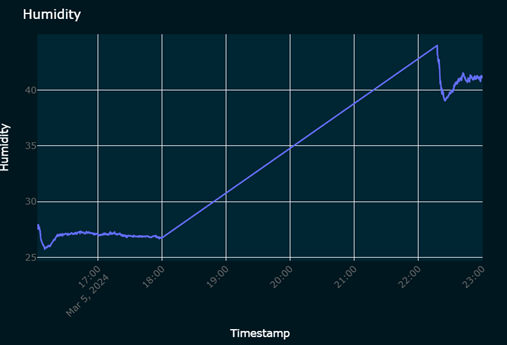
\includegraphics[scale=1]{image/feuchtigkeit.png}
	\caption{Messung Feuchtigkeit}
	\label{fig:enter-label}
\end{figure}
\vspace{3mm}
Hier ist die Veränderung der Luftfeuchtigkeit über die Zeit zu sehen. Zu Beginn der Datenaufnahme wurde die normale Luftfeuchtigkeit des Raumes ohne äußere Einflüsse gemessen (Wert = 20\%). Anschließend wurde der Luftbefeuchter eingeschaltet, was die Luftfeuchtigkeit des Raumes auf 40\% erhöhte.

\subsubsection{Messergebnis Luftdruck}
Der Luftdruck eines Raumes kann verändert werden, indem die Temperatur des Raumes verändert wird. Umso höher die Temperatur eines Raumes ist, desto größer ist der Luftdruck des Raumes. Somit kann der Luftdruck auf die gleiche Weise wie die Temperatur beeinflusst werden.
\vspace{3mm}
\begin{figure}[H]
	\centering
	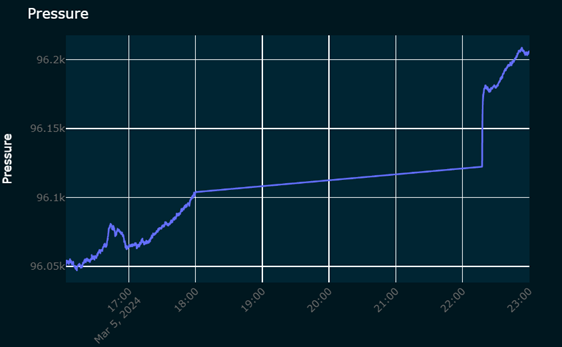
\includegraphics[scale=1]{image/druck.png}
	\caption{Messung Druck}
	\label{fig:enter-label}
\end{figure}
\vspace{3mm}
Oben zu sehen ist die Veränderung des Luftdrucks über die Zeit. Die Korrelation des Luftdrucks und der Temperatur ist dabei gut zu sehen. \\
\vspace{3mm}
Der Luftdruck kann mit folgender Formel berechnet werden: \\
\vspace{3mm}
\begin{figure}[H]
	\centering
	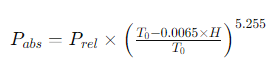
\includegraphics[scale=1.1]{image/formel.png}
	\caption{Formel Druck}
	\label{fig:enter-label}
\end{figure}
Dabei ist:
\begin{itemize}
	\item Pabs der[H] absolute Luftdruck
	\item Prel der relative Luftdruck
	\item H die Höhe in Metern über dem Meeresspiegel
	\item T0 die Standardtemperatur auf Meereshöhe in Kelvin
\end{itemize}
\newpage
Die Messung wurde in Klaus, mit einer Höhe von etwa 507 m. ü. A. (Meter über Adria) durchgeführt. Als relativer Luftdruck wird der Luftdruck am Meeresspiegel verwendet (1013.25 hPa). Anschließend kann der Luftdruck berechnet werden:\\
\vspace{3mm}
\begin{figure}[H]
	\centering
	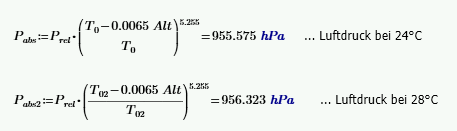
\includegraphics[scale=1.2]{image/berechnung.png}
	\caption{Druckberechnung}
	\label{fig:enter-label}
\end{figure}
\vspace{3mm}
Der berechnete Wert und der gemessene Wert weichen um ca. 5 hPa ab. Der Grund dafür ist, dass die Luftfeuchtigkeit, welche für die Messung künstlich erhöht wurde, in der Rechnung nicht berücksichtigt wurde.

\subsubsection{Messergebnis des UV-Sensors}
Eine Veränderung der UV-Strahlung lässt sich durch langes Messen (ca. ein Tag) gut beobachten. Vor allem lässt sich die Veränderung der UVA-Strahlung (siehe: Kap.: \ref{messuv}) erkennen. Die Messung des UV-Index gestaltet sich zu dieser Jahreszeit (stand: 5.03.2024) jedoch schwierig.\\
\vspace{3mm}
\begin{figure}[H]
	\centering
	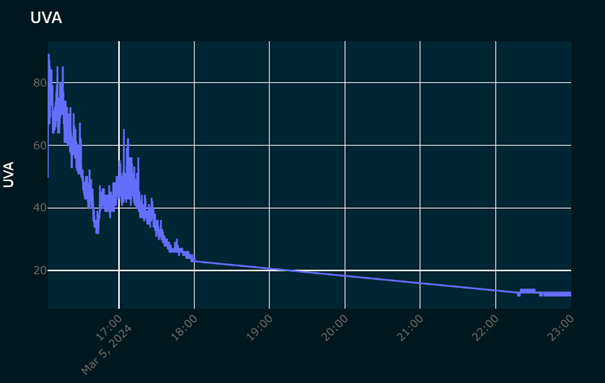
\includegraphics[scale=1]{image/uvamessung.png}
	\caption{Messung UV}
	\label{fig:enter-label}
\end{figure}
\vspace{3mm}
Zu sehen ist die Veränderung der UVA-Strahlung über eine Zeit von 7 Stunden. Die Sonne ging zu dieser Zeit des Jahres um etwa 18:30 Uhr unter, was auch bedeutet, dass die Sonnenstrahlung schwächer wird. 

\subsubsection{Messergebnis der Geschwindigkeit und des Gyroskops}
Sowohl das Gyroskop als auch der Geschwindigkeitssensor können auf die gleiche Weise getestet werden. Durch Drehung des Sensorbretts oder des CubeSats kann eine Bewegung durch die Schwerkraft simuliert werden.\\
\vspace{3mm}
\begin{figure}[H]
	\centering
	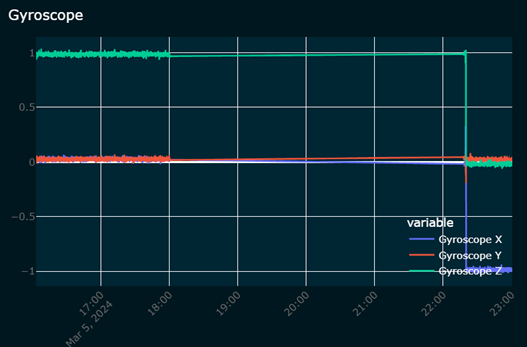
\includegraphics[scale=1]{image/messgyros.png}
	\caption{Messung Gyroskop}
	\label{fig:enter-label}
\end{figure}
\vspace{3mm}
Hier sehen Sie den gyroskopischen, magnetischen Sensor BMM150. Es ist zu erkennen, dass für die gyroskopische Messung drei Achsen verwendet werden. Zunächst ist der Wert Z auf eins, was auf die Orientierung des Sensors in Richtung der Z-Achse hinweist. Anschließend um etwa 22:30 Uhr wurde der CubeSat auf seine X-Achse gestellt.